\documentclass{beamer}  
\usepackage[T1]{fontenc}
\usepackage{xcolor}
\usepackage{mathtools}
\usepackage{graphicx}
\usepackage{subcaption}

\usefonttheme[onlymath]{serif}
\renewcommand\sfdefault{cmtt}

\usecolortheme[named=black]{structure}
\setbeamercolor{normal text}{fg=black}
\setbeamercolor{structure}{fg=black}
\setbeamercolor{section in toc}{fg=black}

\title{intro to mathematics in software engineering}
\institute{Fontys University of Applied Sciences}
\date{\today}

\begin{document}
	
	% title-page
	\begin{frame}
		\titlepage
	\end{frame}
	
	% objectives
	\begin{frame}{objectives}
		\begin{itemize}
			\item[] scary looking functions
			\item[] math related software engineering concepts
			\item[] translate math to programming
		\end{itemize}
	\end{frame}
	
	% fundamentals-1
	\begin{frame}{fundamentals of mathematical and function notation}
		$$f(x)=x^2$$
	\end{frame}
	
	% fundamentals-2
	\begin{frame}{fundamentals of mathematical and function notation}
		\begin{itemize}
			\item[] $a\cdot f(x)$
			\item[]
			\item[] $f(x/b)$
			\item[]
			\item[] $f(x-c)$
			\item[]
			\item[] $f(x)+d$
		\end{itemize}
	\end{frame}
	
	% fundamentals-3
	\begin{frame}{fundamentals of mathematical and function notation}
		\begin{itemize}
			\item[] $a\cdot f(x) \Rightarrow \text{multiplies the y-value by } a$
			\item[]
			\item[] $f(x/b) \Rightarrow \text{multiplies the x-value by } b$
			\item[]
			\item[] $f(x-c) \Rightarrow \text{shifts graph } c \text{ units to the right}$
			\item[]
			\item[] $f(x)+d \Rightarrow \text{shifts graph } d \text{ units upward}$
		\end{itemize}
	\end{frame}

	% breakdown-1
	\begin{frame}{breaking down a scary looking function}
		\vfill
		\begin{center}
			$$g(x)=\frac{4}{\pi}\sum_{n=1}^{\infty}\frac{\sin(2\pi (2n-1)ft)}{2n-1}$$
		\end{center}
		\vfill
		\begin{center}
			\small (where $t = \text{time},\ f = \text{frequency},\ n = \text{iterations}$)
		\end{center}
		\vfill
	\end{frame}

	
	% breakdown-2
	\begin{frame}{breaking down a scary looking function}
		\vfill
		\begin{center}
			$$g(x) = \frac{4}{\pi}\colorbox{red!20}{$\displaystyle \sum_{n=1}^{\infty}$}\frac{\sin(2\pi(2n-1)ft)}{2n-1}$$
		\end{center}
		\vfill
		\begin{center}
			we are dealing with a function built from multiple smaller functions added together
		\end{center}
		\vfill
	\end{frame}

	
	% breakdown-3
	\begin{frame}{breaking down a scary looking function}
		\vfill
		\begin{center}
			$$g(x)=\frac{4}{\pi}\sum_{n=1}^{\infty}\frac{\colorbox{red!20}{$\displaystyle \sin$}(2\pi (2n-1)ft)}{2n-1}$$
		\end{center}
		\vfill
		\begin{center}
			the $sin$ on the inside suggests we are dealing with waves or oscillations
		\end{center}
		\vfill
	\end{frame}
	
	% breakdown-4
	\begin{frame}{breaking down a scary looking function}
		\vfill
		\begin{center}
			$$g(x)=\frac{4}{\pi}\sum_{n=1}^{\infty}\frac{\sin(2\pi (2n-1)ft)}{\colorbox{red!20}{$\displaystyle 2n-1$}}$$
		\end{center}
		\vfill
		\begin{center}
			denominator \(2n-1\) hints that terms get smaller as \(n\) increases — later terms have less influence
		\end{center}
		\vfill
	\end{frame}

	
	% breakdown-5
	\begin{frame}{breaking down a scary looking function}
		$$g_{1}(t)=\frac{4}{\pi}\cdot \frac{\sin(2\pi (2(1)-1)ft)}{2(1)-1}$$
		$$=\frac{4}{\pi}\cdot \frac{\sin(2\pi (1)ft)}{1}$$
		$$=\frac{4}{\pi}\cdot\sin(2\pi ft)$$
		$$g_{1}(t)=\colorbox{green!20}{$\displaystyle \frac{4}{\pi}\sin(2\pi ft)$}$$
	\end{frame}
	
	% breakdown-6
	\begin{frame}{breaking down a scary looking function}
		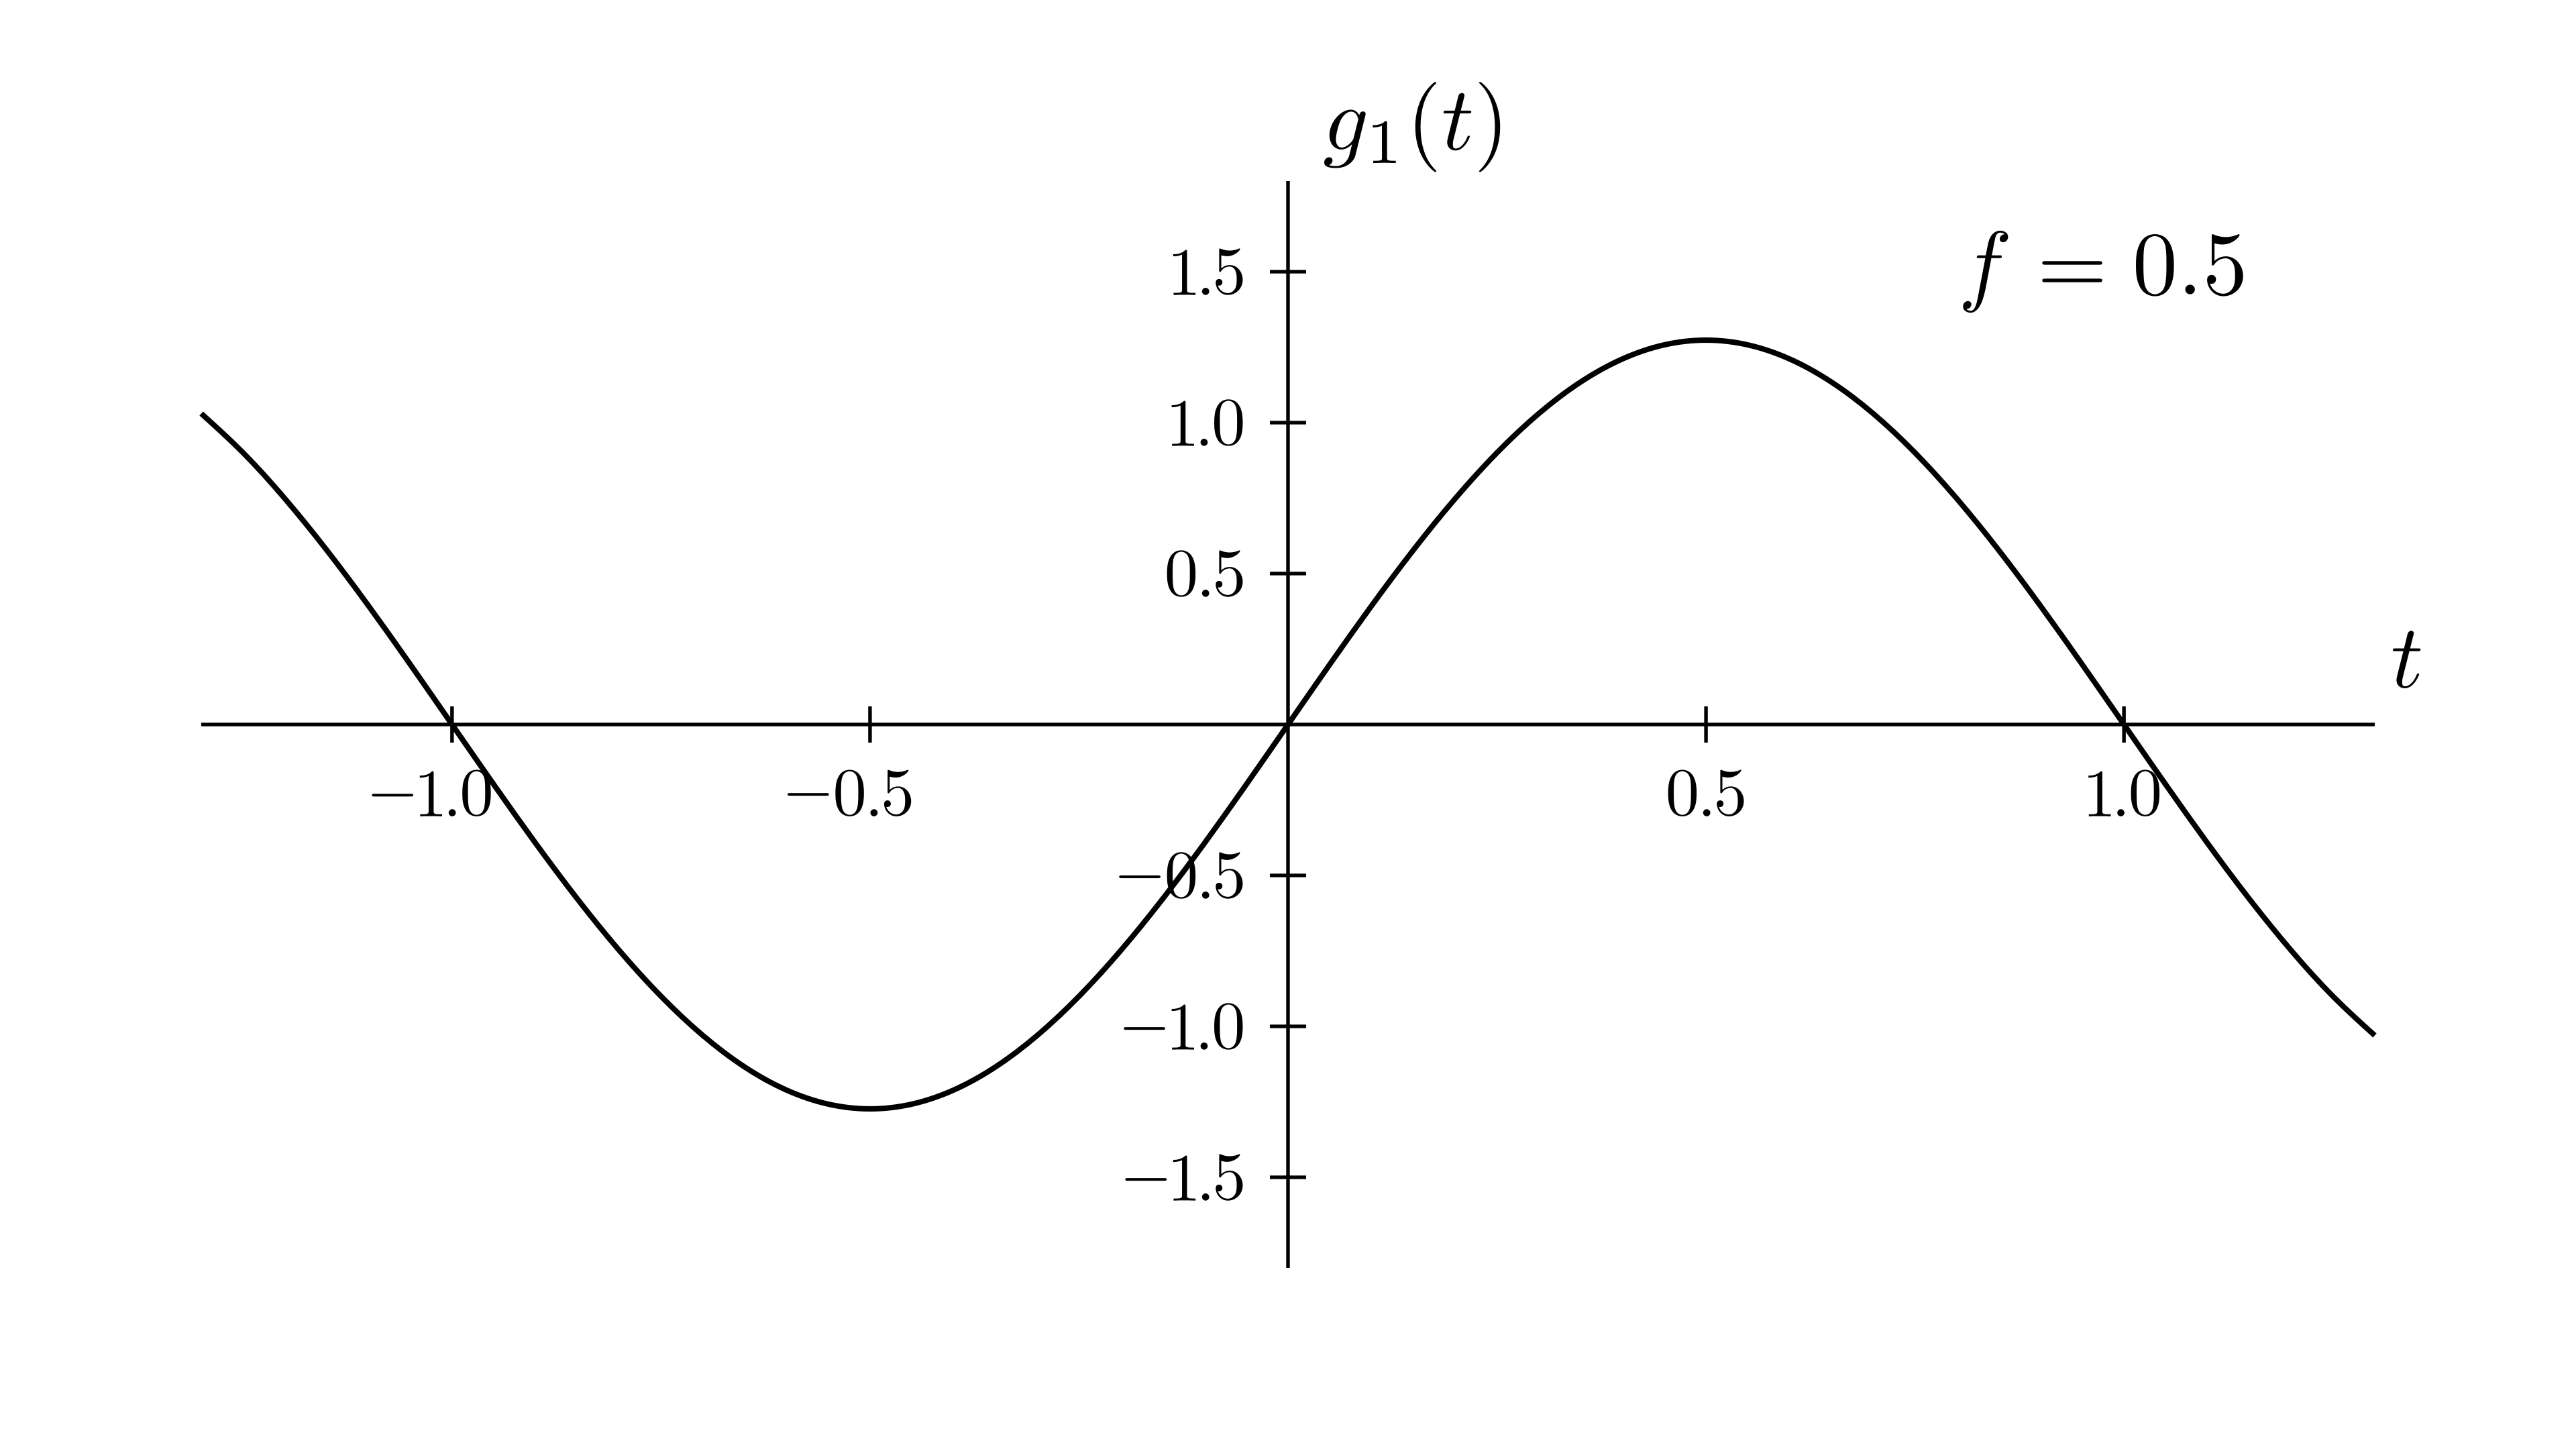
\includegraphics[width=\linewidth,height=0.85\textheight,keepaspectratio]{../assets/first-term-function.png}
	\end{frame}

	% breakdown-7
	\begin{frame}{breaking down a scary looking function}
		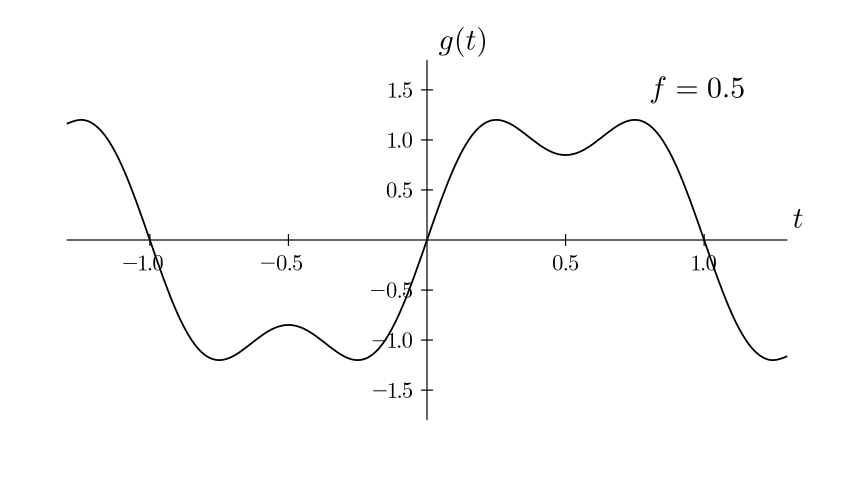
\includegraphics[width=\linewidth,height=0.85\textheight,keepaspectratio]{../assets/second-term-function.png}
	\end{frame}
	
	% breakdown-8
	\begin{frame}{breaking down a scary looking function}
		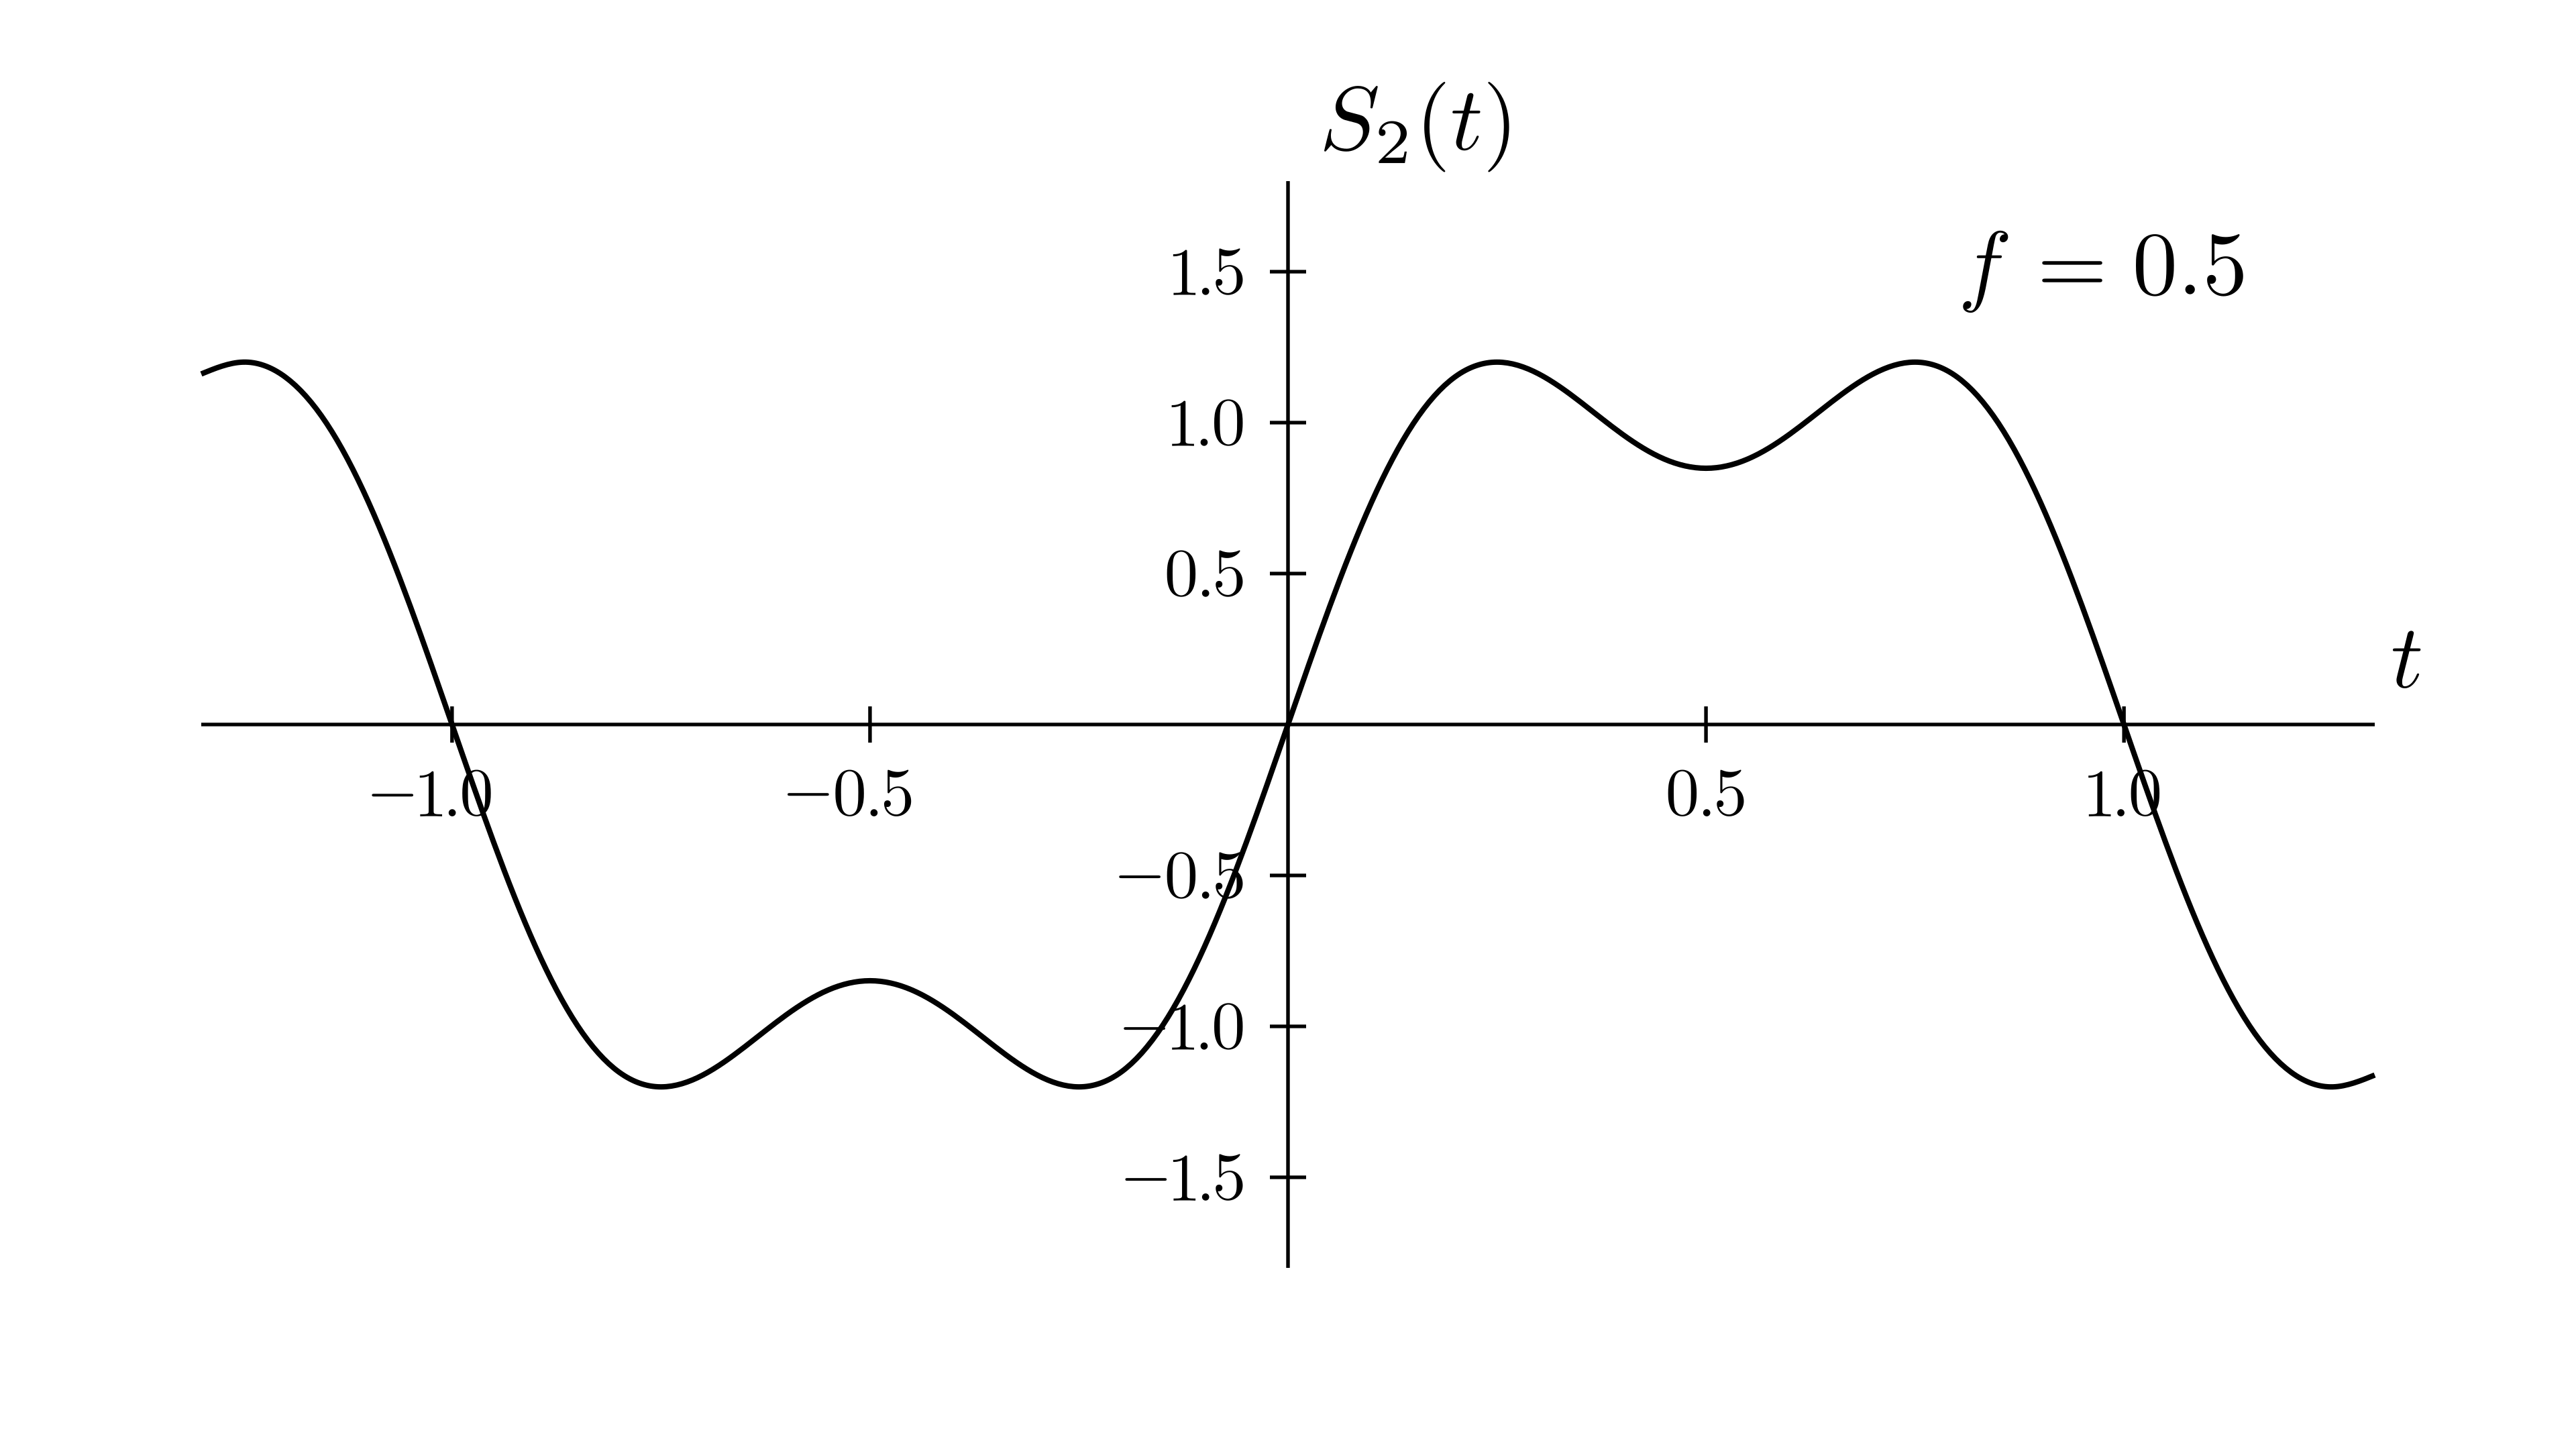
\includegraphics[width=\linewidth,height=0.85\textheight,keepaspectratio]{../assets/sum-two-terms.png}
	\end{frame}
	
	% breakdown-9
	\begin{frame}{breaking down a scary looking function}
		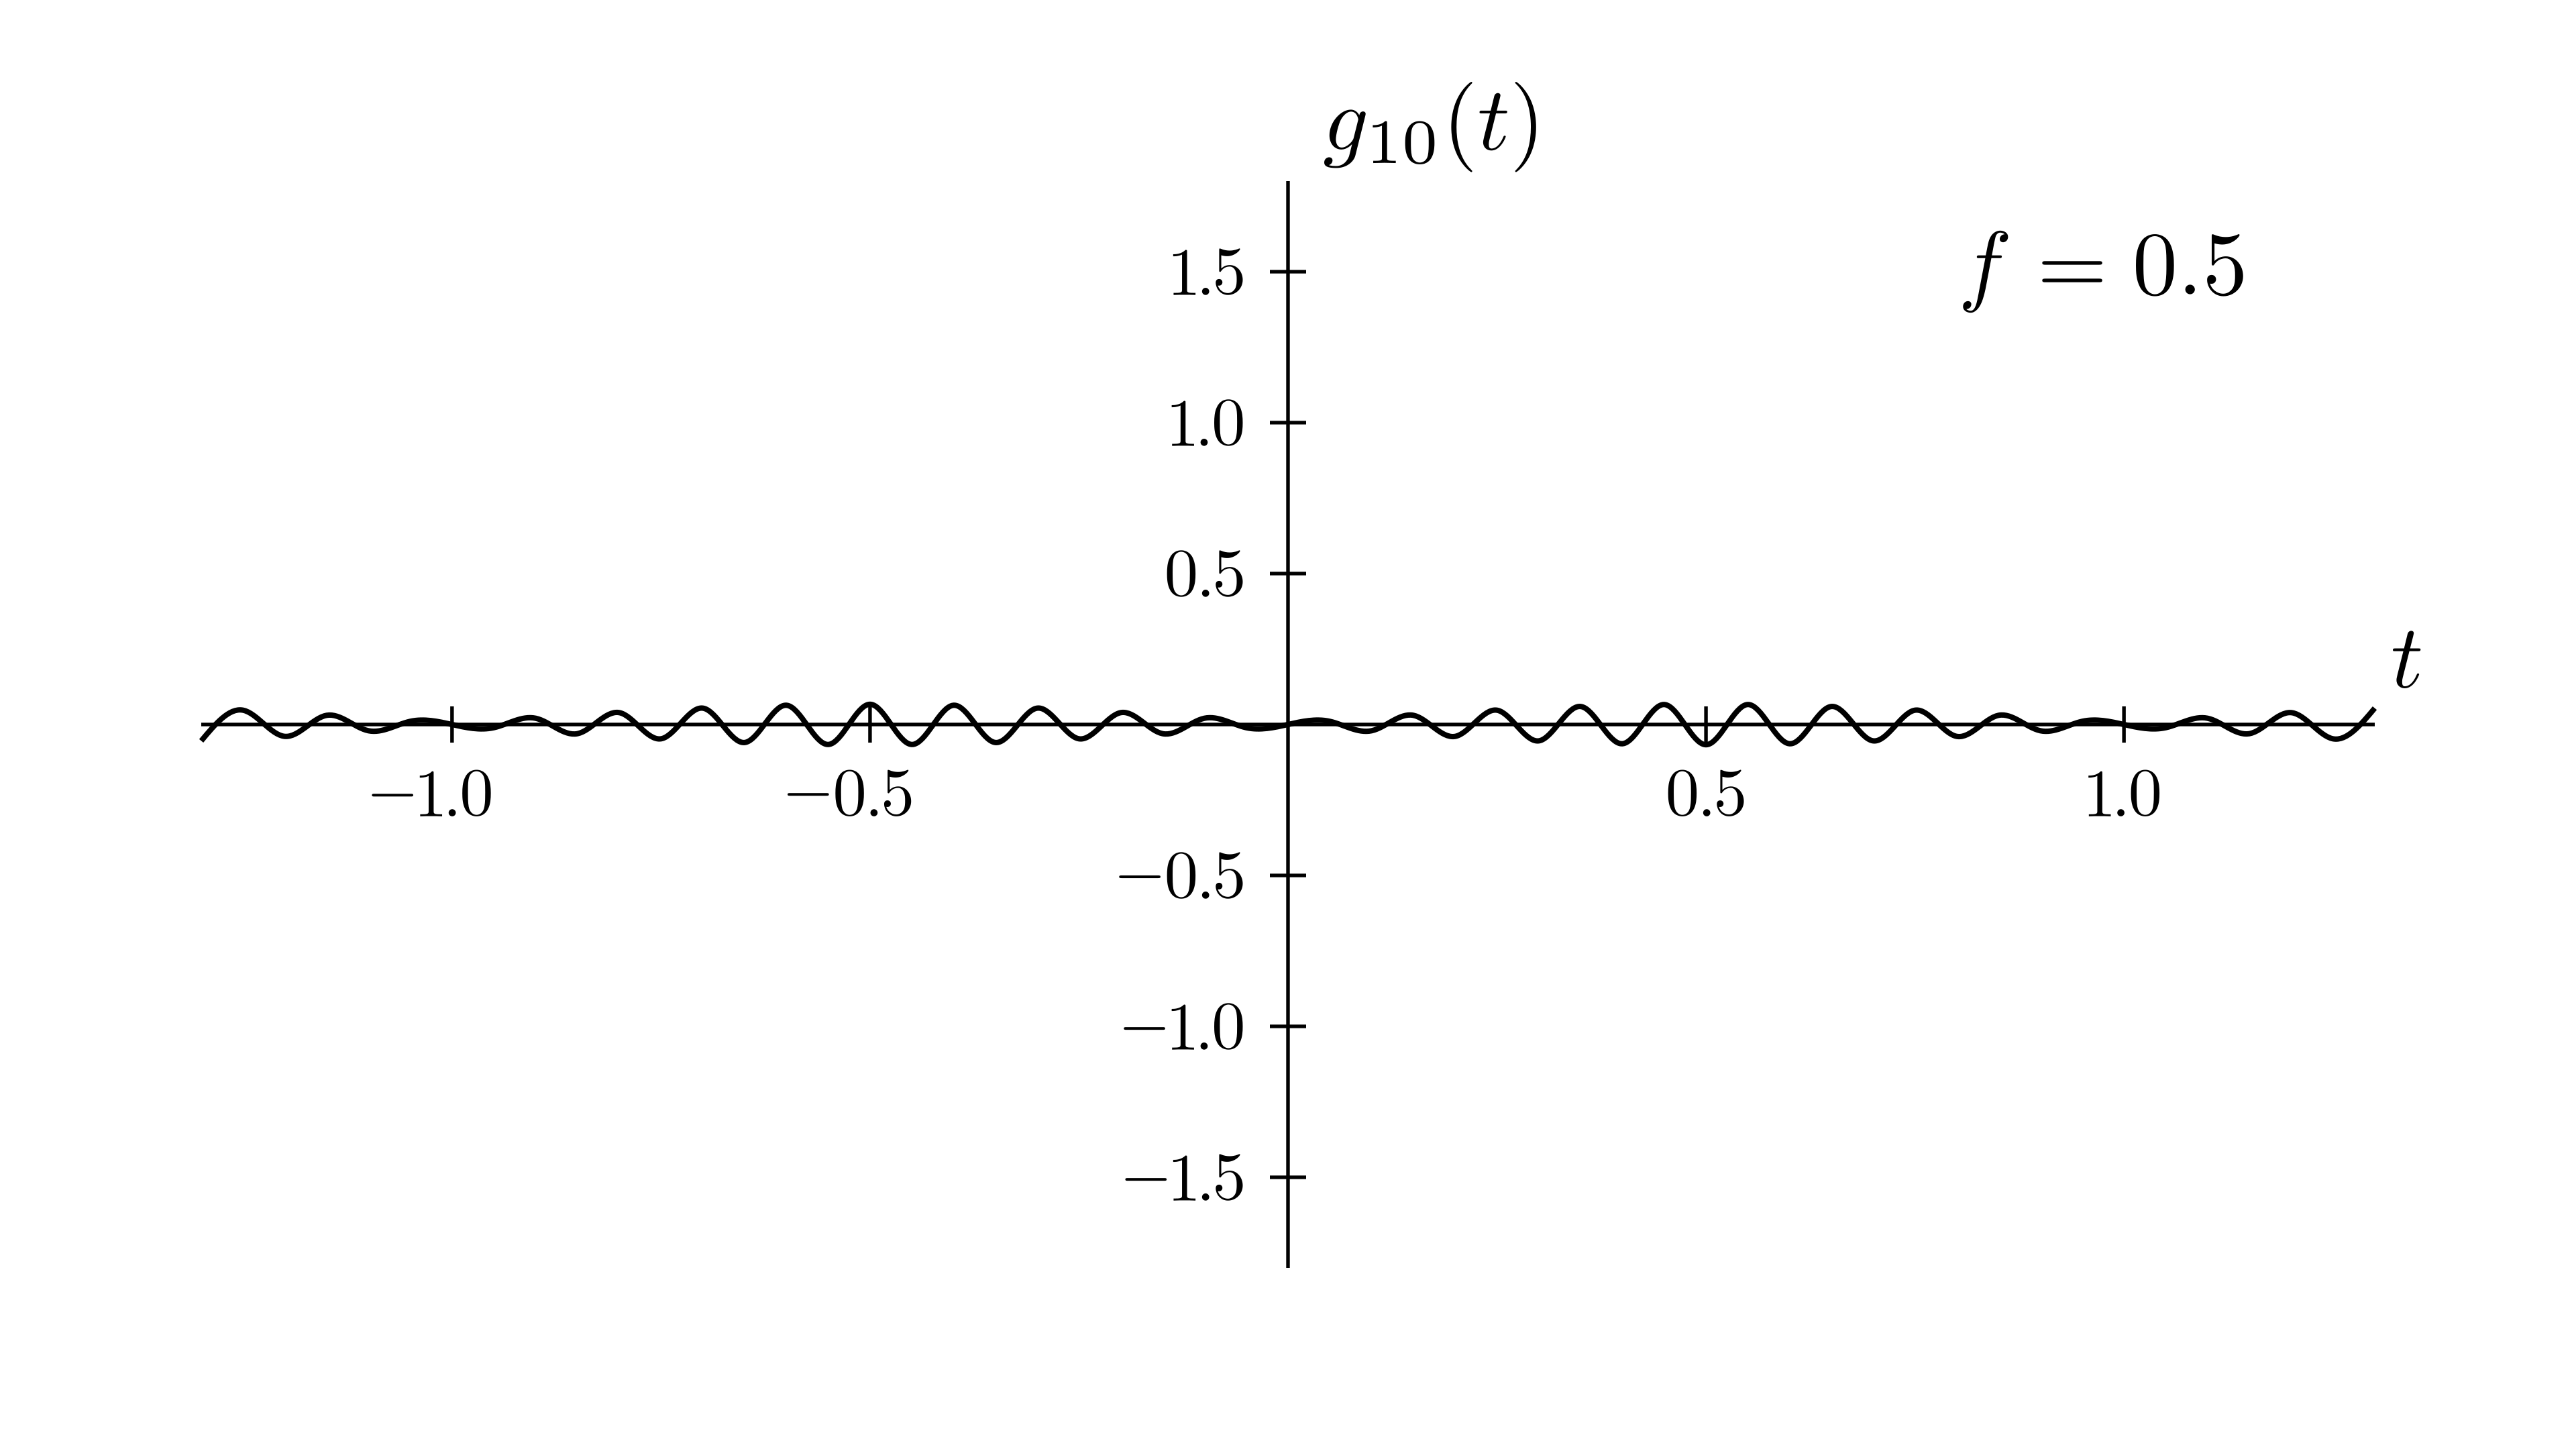
\includegraphics[width=\linewidth,height=0.85\textheight,keepaspectratio]{../assets/tenth-term-function.png}
	\end{frame}
	
	% breakdown-10
	\begin{frame}{breaking down a scary looking function}
		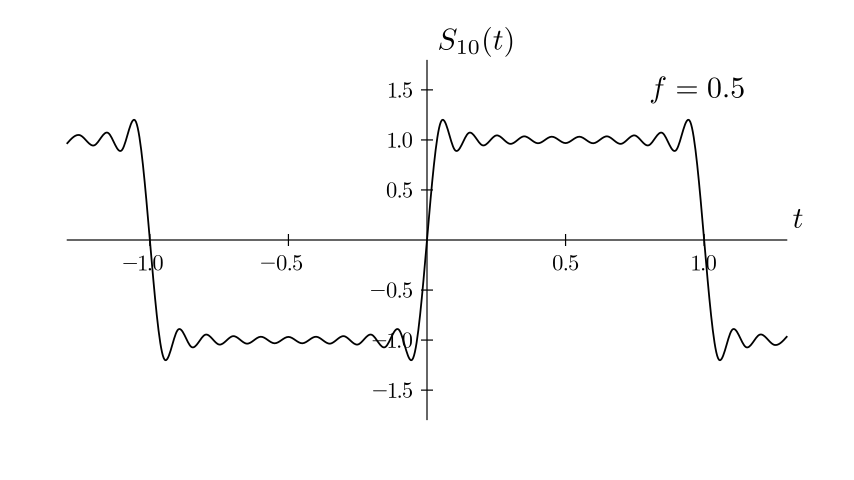
\includegraphics[width=\linewidth,height=0.85\textheight,keepaspectratio]{../assets/sum-ten-terms.png}
	\end{frame}
	
	% arrays-1
	\begin{frame}{vectors (not the math kind), i.e. arrays}
		\begin{itemize}
			\item[] set of pairs $\Rightarrow$ index and value
			\item[] elements (pairs) are conventionally of same memory size
		\end{itemize}
	\end{frame}
	
	% arrays-2
	\begin{frame}{vectors (not the math kind), i.e. arrays}
		\vfill
		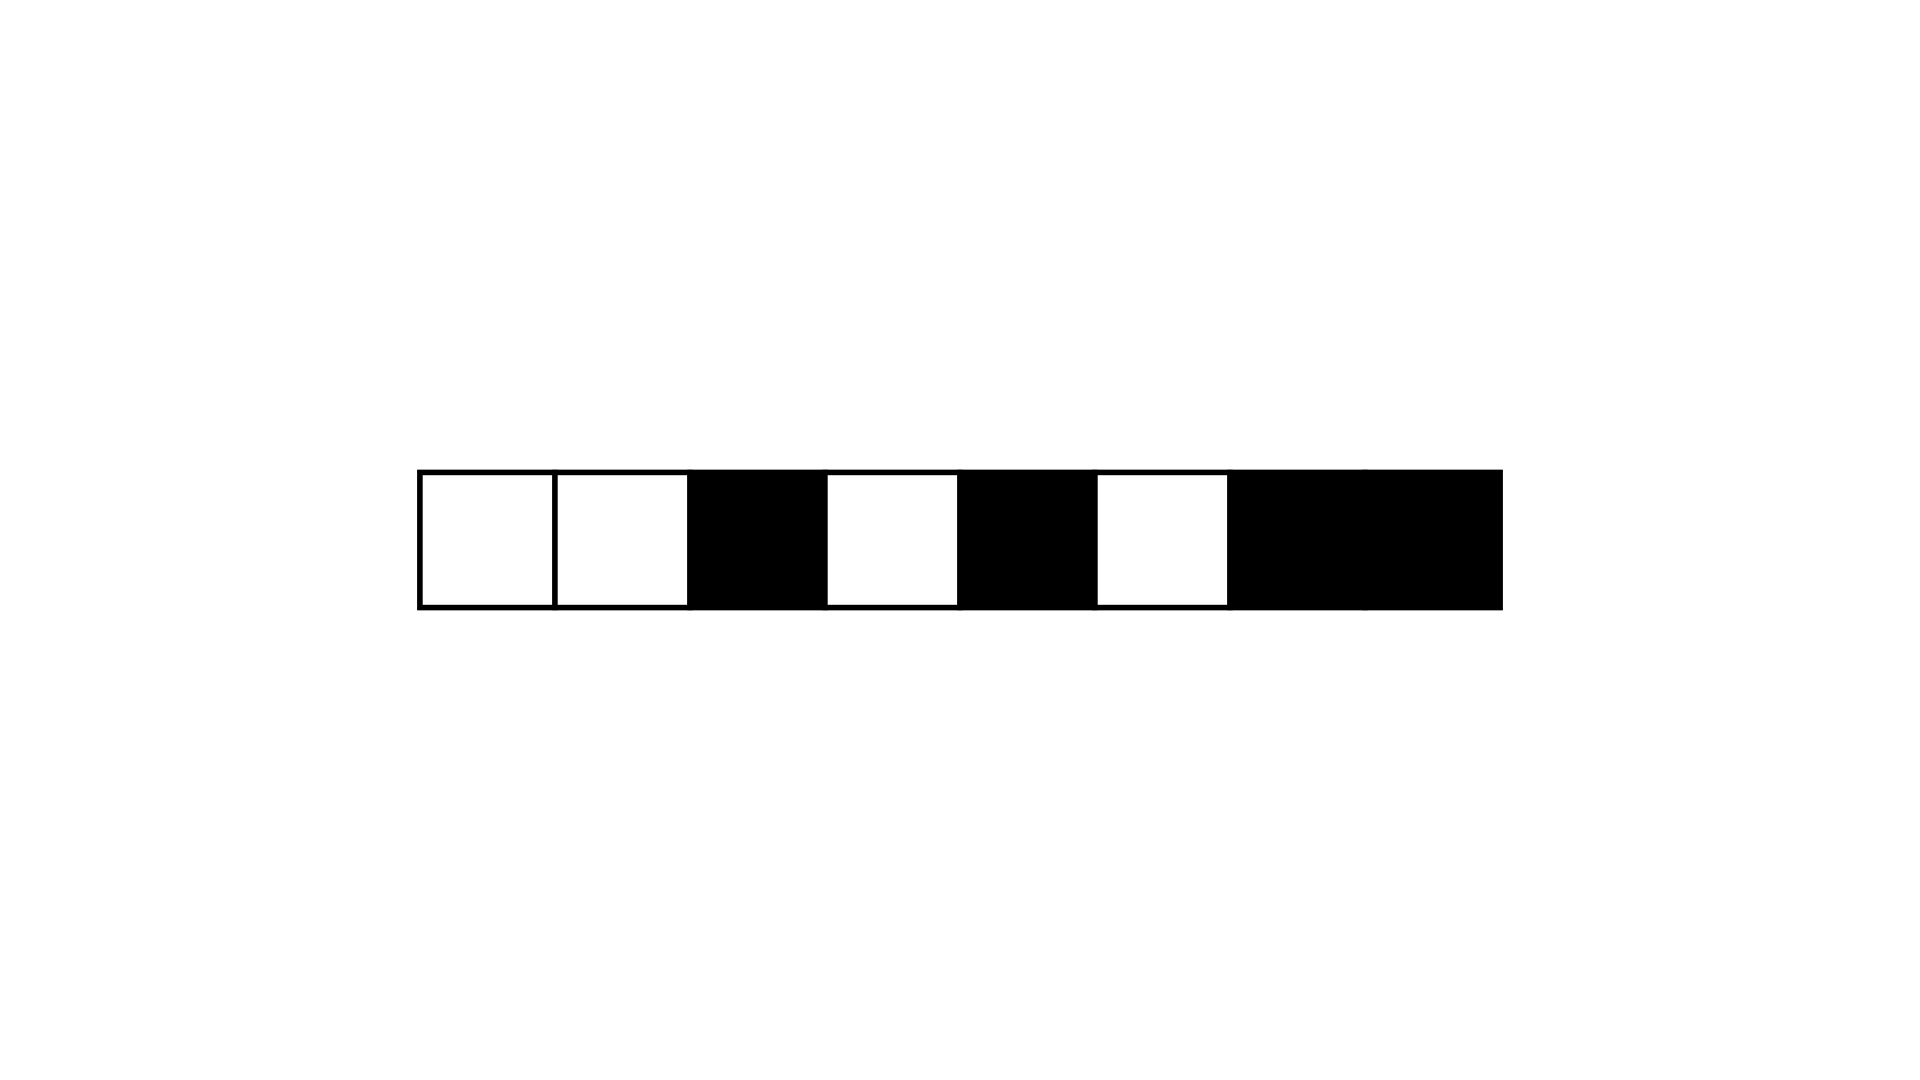
\includegraphics[width=\linewidth,height=0.85\textheight,keepaspectratio]{../assets/1d-array.png}
		\vfill
		\small
			one\_d\_array = [0, 0, 1, 0, 1, 0, 1, 1]
		\vfill
	\end{frame}
	
	% arrays-3
	\begin{frame}{vectors (not the math kind), i.e. arrays}
		\vfill
		
\includegraphics[width=\linewidth,height=0.85\textheight,keepaspectratio]{../assets/2d-array.png}
		\vfill
	\end{frame}
	
	% arrays-4
	\begin{frame}{vectors (not the math kind), i.e. arrays}
		\vfill
		\small
			two\_d\_array = [
			
			[0, 0, 0, 0, 0, 0, 0, 0],
			
			[0, 0, 1, 0, 0, 1, 0, 0],
			
			[0, 0, 1, 0, 0, 1, 0, 0],
			
			[0, 0, 1, 0, 0, 1, 0, 0],
			
			[0, 0, 0, 0, 0, 0, 0, 0],
			
			[0, 1, 0, 0, 0, 0, 1, 0],
			
			[0, 0, 1, 1, 1, 1, 0, 0],
			
			[0, 0, 0, 0, 0, 0, 0, 0]
			
		]
		\vfill
	\end{frame}
	
	% arrays-5
	\begin{frame}{vectors (not the math kind), i.e. arrays}
		\begin{center}
			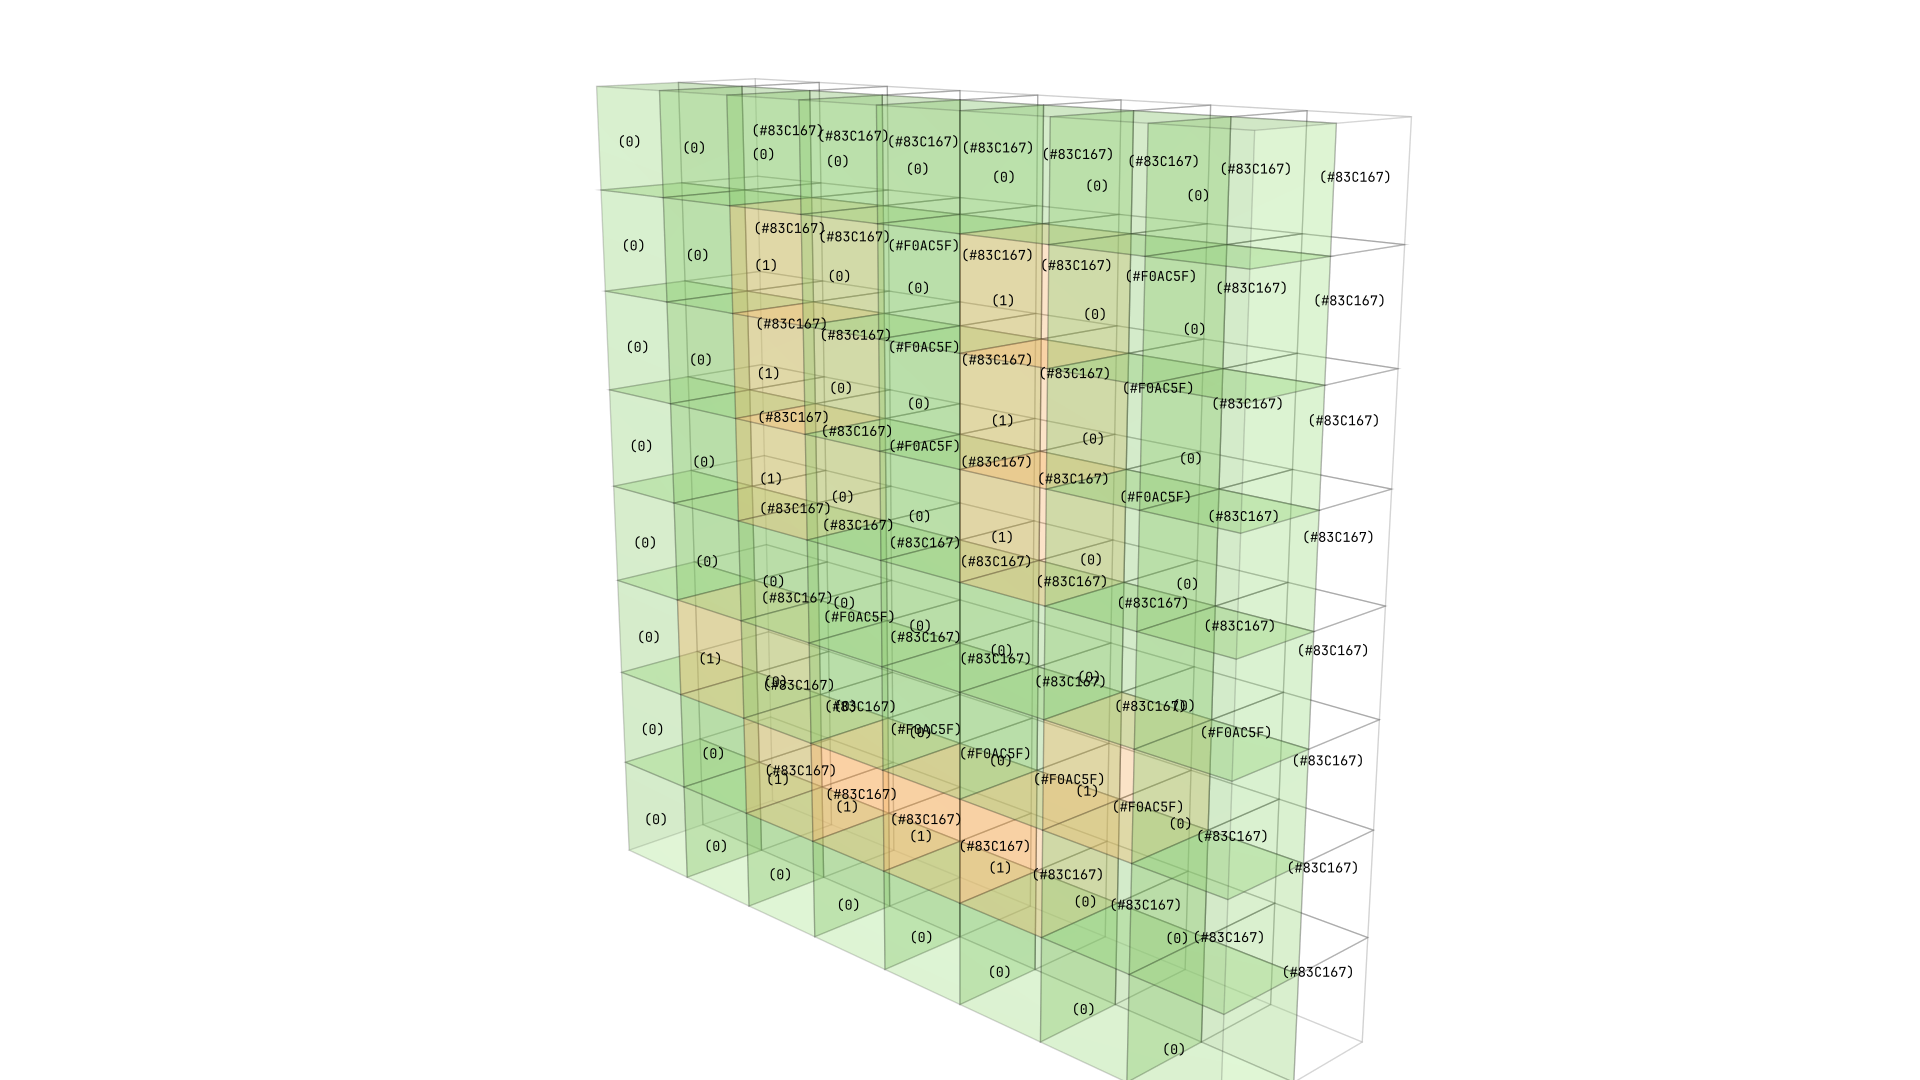
\includegraphics[width=\linewidth,height=0.85\textheight,keepaspectratio]{../assets/3d-array-rotated.png}
		\end{center}
	\end{frame}
	
	\begin{frame}{binary tree}
		\begin{itemize}
			\item[] data structure expressed as a figurative tree
			\item[] one root node
			\item[] nodes can only have one parent node and at most two children nodes (left and right)
			\item[] foundation for more complex data structures
		\end{itemize}
	\end{frame}

\end{document}
